\section{Strona internetowa}
\lstset{language=HTML, inputencoding=utf8, breaklines=true}

Strona interetowa pozwala na zdalny i czytelny podgląd danych, które napływają seriami w czasie rzeczywistym. Dzięki wykorzystaniu strony internetowej, możliwe staje się utworzenie konta użytkownika, przypisanie do niego urządzeń, a następnie podgląd tras - zarówno aktualnie przebywanej jak i historycznych wraz z ich parametrami, zapisanymi na serwerze.

Szkielet strony internetowej został zaprojektowany w języku HTML (\textit{ang. \textbf{H}yper\textbf{t}ext \textbf{M}arkup \textbf{L}anguage}), natomiast jej część funkcjonalna powstała przy użyciu języka \textit{JavaScript}. Jest to wysokopoziomowy, obiektowo-funkcyjny język skryptowy, wykorzystywany głównie w przeglądarkach, charakteryzujący się jednowątkowością.

Dzięki wykorzystaniu JavaScript, możliwe staje się dodanie wielu funkcjonalności do struktury strony internetowej, które stanowią jej połączenie ze światem zewnętrznym oraz umożliwiają wykorzystanie wielu efektownych rozwiązań wizualnych. Są to na przykład animowane przewijanie strony, wyskakujące okienka czy interaktywne wykresy.

W niniejszej pracy język JavaScript został wykorzystany do połączenia strony internetowej z bazą danych w celu użycia wymienionych w poprzednim podrozdziale funkcji, umożliwienia interakcji użytkownika ze stroną internetową, a także wyświetlenia tras na mapie w postaci znaczników oraz przypisanych do nich okienek informacyjnych.  

Na rysunkach \ref{fig:image_soft_website_login}, \ref{fig:image_soft_website_register_user}, \ref{fig:image_soft_website_main_page} oraz \ref{fig:image_soft_website_track_map} przedstawiono podstawowe ekrany: logowania, rejestracji użytkownika, ekran główny oraz ekran trasy.

\begin{figure}[H]
	\centering
	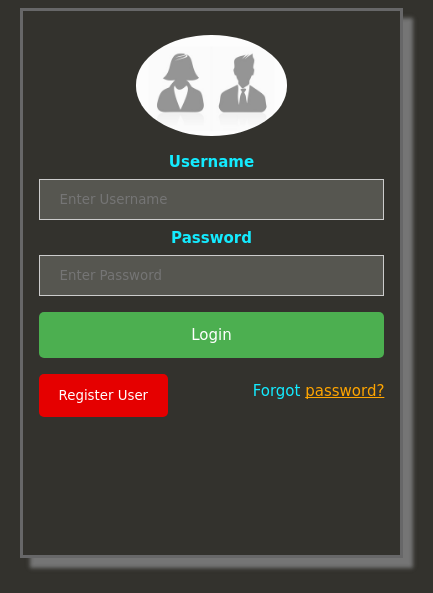
\includegraphics[width=8cm]{img/software/website/login_window.png}
	\caption{Strona logowania. Źródło: Opracowanie własne.}
	\label{fig:image_soft_website_login}
\end{figure}

\begin{figure}[H]
	\centering
	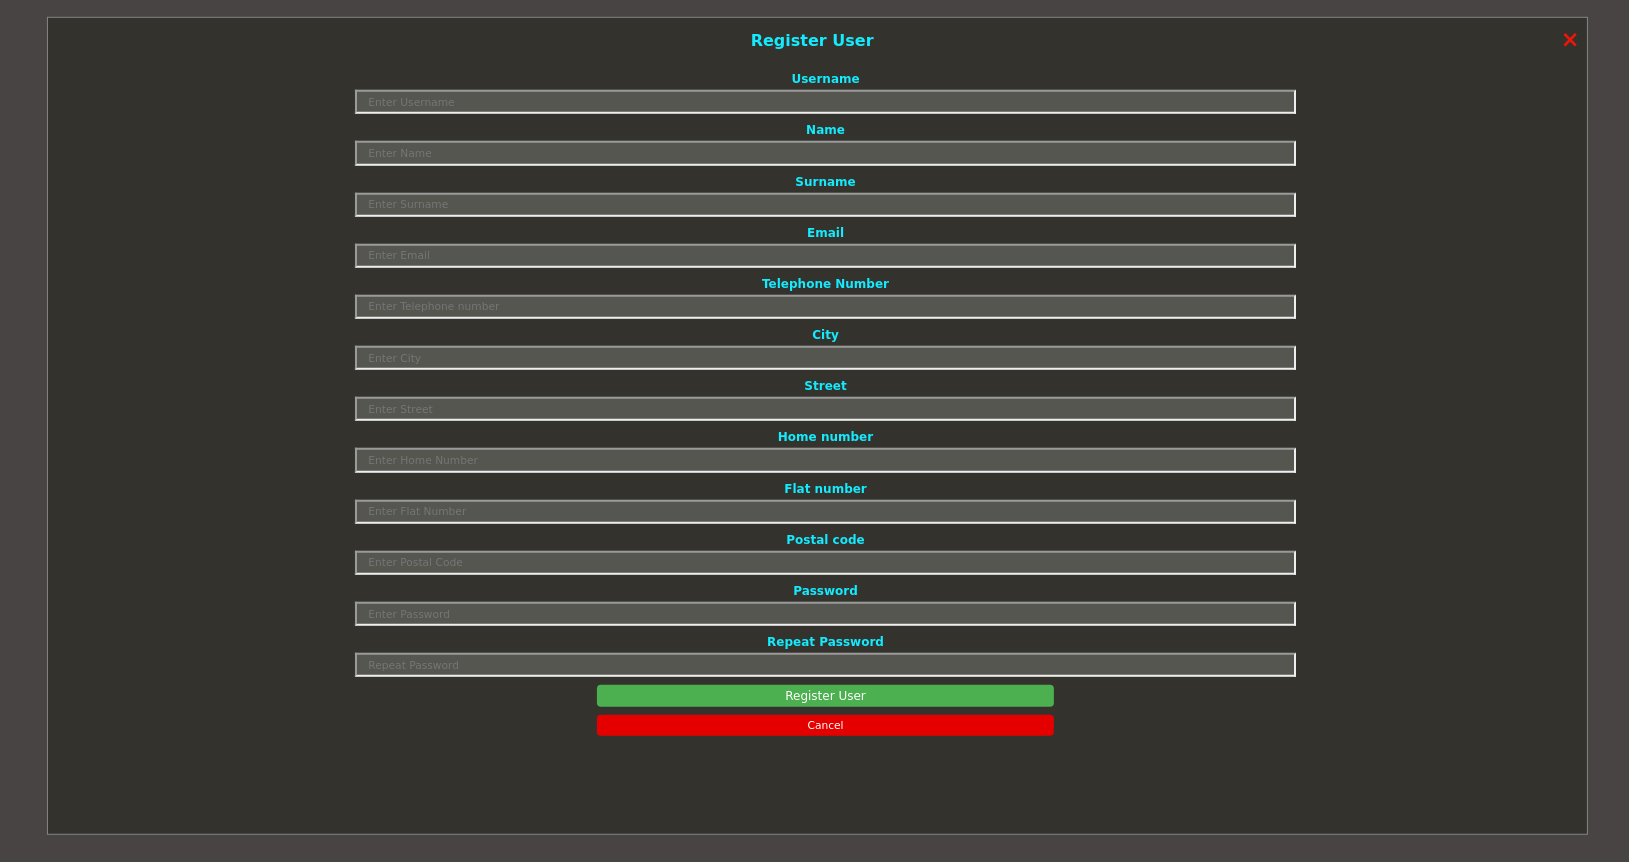
\includegraphics[width=17cm]{img/software/website/register_user.png}
	\caption{Ekran rejestracji użytkownia. Źródło: Opracowanie własne.}
	\label{fig:image_soft_website_register_user}
\end{figure}

\begin{figure}[H]
	\centering
	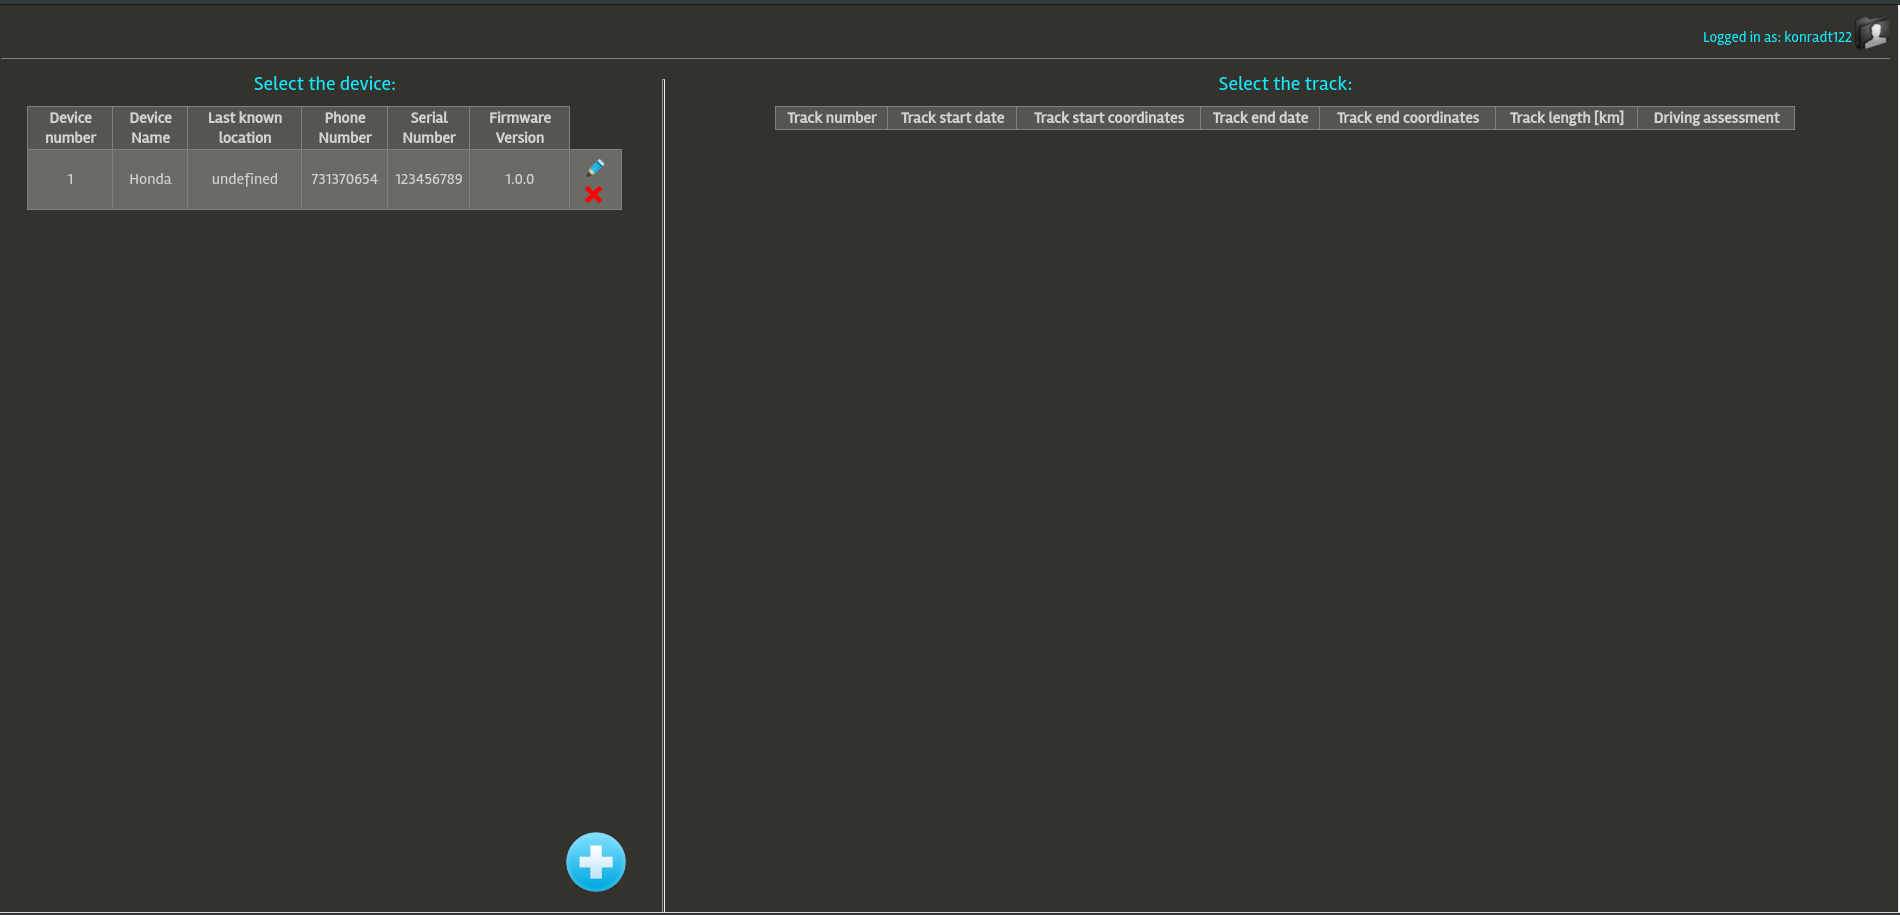
\includegraphics[height=23cm, width=16cm]{img/software/website/main_screen.png}
	\caption{Strona główna. Źródło: Opracowanie własne.}
	\label{fig:image_soft_website_main_page}
\end{figure}

\begin{figure}[H]
	\centering
	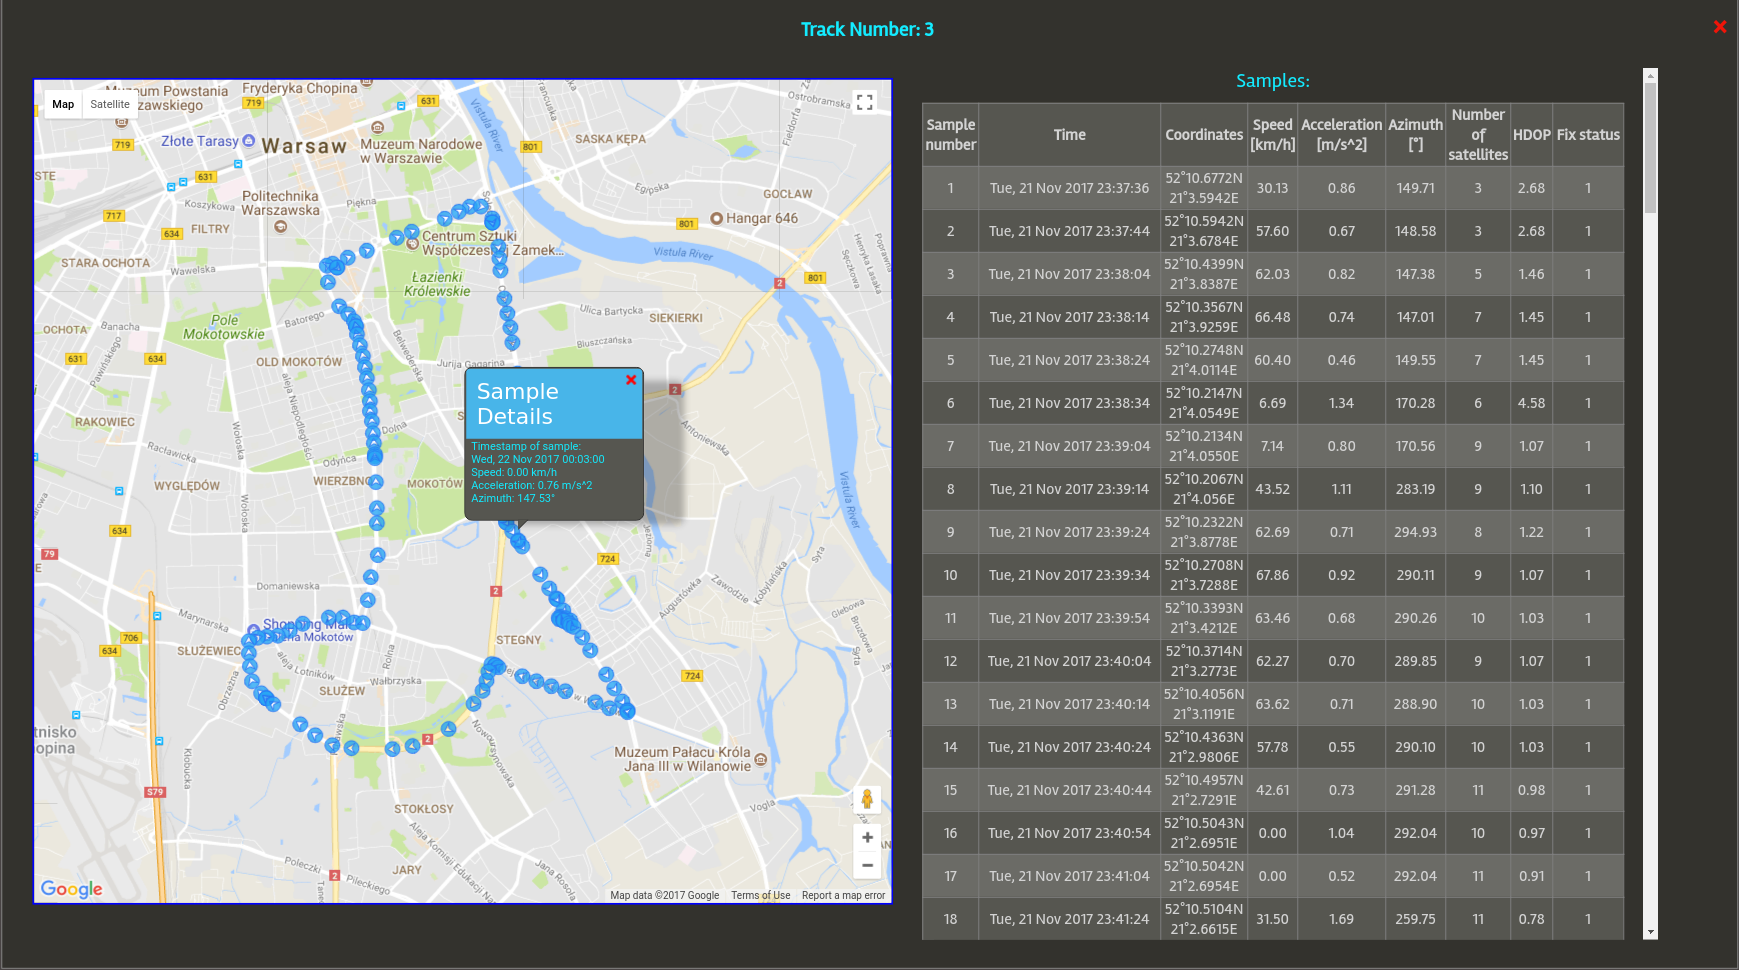
\includegraphics[height=23cm, width=16cm]{img/software/website/track_modal.png}
	\caption{Okno trasy. Źródło: Opracowanie własne.}
	\label{fig:image_soft_website_track_map}
\end{figure}

\clearpage
Ekran trasy przedstawia poszczególne próbki lokalizacji, należące do trasy, na mapie od firmy Google. W tym celu, niezbędne staje się wykorzystanie API producenta dla modułu Google Maps. Pozwala ono na wyświetlenie mapy, przybliżanie i oddalanie, odnalezienie lokalizacji, naniesienie znaczników (w tym autorskich - zdefiniowanych w formacie grafiki wektorowej - \textit{.svg}). Ponadto, dzięki zastosowaniu modułu \textit{Info Bubble}, możliwe staje się wyświetlenie na mapie interaktywnego okienka informacyjnego, powiązanego z konkretnym znacznikiem geolokalizacyjnym.

Aby wykorzystać API Google Maps, należy zarejestrować aplikację na stronie \url{https://developers.google.com/maps/documentation/javascript/get-api-key}. Po rejestracji, do projektu przypisany zostanie klucz, który należy zawrzeć wewnątrz zapytania HTTP wykonywanego przy ładowaniu strony, umożliwiającego ściągnięcie z internetu plików źródłowych zawierających kod obsługujący mapy. Przedstawiono to na listingu \ref{listing_google_map_api}.

\begin{lstlisting}[label=listing_google_map_api, caption=Fragment kodu pozwalający na użycie API Google Maps]
<script async defer src="https://maps.googleapis.com/maps/api/js?key=TWOJ_KLUCZ_API&callback=initMap" type="text/javascript"></script>
\end{lstlisting}

